\icode{N19-EME-SI-L2-261121-003}
\nceeID[6]{2019全国\Rmnum{1}}{15}
如图，空间存在一方向水平向右的匀强电场，两个带电小球\(P\)和\(Q\)用相同的绝缘细绳悬挂在水平天花板下，两细绳都恰好与天花板垂直，则\paren[]

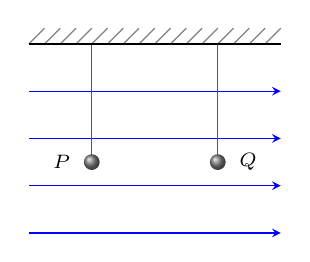
\begin{tikzpicture}[>=stealth,font=\scriptsize]
	\foreach \y in {-2.4,-1.8,...,-.4}
		\draw[->,blue] (-1.6,\y)--(1.6,\y);
	\draw[magenta] (-.8,0)--(-.8,-1.5) (.8,0)--(.8,-1.5);
	\shade[ball color=gray] (-.8,-1.5) circle(.1);
	\shade[ball color=gray] (.8,-1.5) circle(.1);
	\foreach \x in {-1.6,-1.4,...,1.6}
		\draw[gray] (\x,0)--++(.2,.2);
	\draw[thick] (-1.6,0)--(1.6,0);
	\node at(-.95,-1.5)[left]{\(P\)};
	\node at(.95,-1.5)[right]{\(Q\)};
\end{tikzpicture}
\begin{choices}
	\item \(P\)和\(Q\)都带正电荷
	\item \(P\)和\(Q\)都带负电荷
	\item \(P\)带正电荷，\(Q\)带负电荷
	\item \(P\)带负电荷，\(Q\)带正电荷
\end{choices}
\begin{answer}
	D\qquad 提示：
\end{answer}